\documentclass[11pt]{article}
\usepackage{graphicx} % Required for inserting images
\usepackage[top=2.5cm, bottom=2.5cm, left=2.5cm, right=2.5cm]{geometry}
\usepackage[T1]{fontenc}
\usepackage{hyperref}
\usepackage[utf8]{inputenc}
\usepackage{multirow}
\usepackage{subcaption}
\usepackage{booktabs}
\usepackage{bookmark}
\usepackage{graphicx}
\usepackage{setspace}
\setlength{\parindent}{0in}
\usepackage{physics}
\usepackage{tikz}
\usepackage{tikz-3dplot}
\usepackage[outline]{contour} % glow around text
\usepackage{xcolor}
\usepackage{float}
\usepackage{makeidx}
\usepackage{fancyhdr}
\usepackage{pgfplots}
\usepackage{amsmath}
\pgfplotsset{compat=1.18}
\usepackage{caption}
\usepackage[english,catalan]{babel}
\setlength{\parskip}{11pt}
\usepackage{xcolor}
\usepackage{listings}
\usepackage{marginnote}
\usepackage{siunitx}


\title{\Huge\bfseries Pràctica de simulació: \\ Instal·lació de panells solars fotovoltaics en un habitatge unifamiliar a Catalunya \\ [2ex] \Large}

\author{\begin{tabular}{c}
\textbf{GRUP C3} \\
Isaac Baldi García (1667260)\\
Marcel López Freixes (1668323) \\
Eira Jacas García (1666616) \\
Núria Castillo Ariño (1669145)
\end{tabular}}

\date{Gener 2025}

\begin{document}

\maketitle
\begin{center}
    \textbf{Resum:} Aquest informe és un anàlisi sobre la instal·lació de panells solars fotovoltaics en un habitatge a Catalunya. Es modelitza el moviment orbital de la Terra per determinar la trajectòria solar respecte a l’habitatge, resolent l’equació del moviment amb diferents mètodes numèrics per comparar-ne l’eficiència. Amb aquestes dades, es calcula la potència i l’energia generades pel panell solar i es determina la configuració òptima per maximitzar la producció energètica. Finalment, al model s'hi incorpora la forma no esfèrica de la Terra, per tal d'ajustar-lo més a la realitat.
\end{center}


\newpage

\tableofcontents
\newpage



\section{Moviment de la Terra al voltant del Sol} \label{sec: seccio_1}
En aquesta secció ens hem proposat simular el moviment de translació de la Terra al voltant del Sol. Per fer-ho hem partit de la Llei de la Gravitació Univeral i hem simplificat el nostre problema de dos cossos a un d'un sol cos sota una força central
\begin{equation}
    F(r)=-\frac{GMm}{r^2}
    \label{si}
\end{equation}
on G és la constant de gravitació universal, M la massa del Sol i m la massa de la Terra.\footnote{Totes les dades orbitalàries agafades del Jet Propulsion Laboratory de la NASA: \url{https://ssd.jpl.nasa.gov/}}

Per aquest tipus de sistemes i considerant únicament aquesta força central, obtenim les següents tres EDOs de primer ordre normalitzades que descriuen el moviment de la Terra (veure deducció matemàtica a l'annex \ref{annex: equ_mov}).
\begin{equation}
    \frac{\partial\tilde{v}}{\partial\tilde{t}}=-\frac{1}{\tilde{r}^2}+\frac{1}{\tilde{r}^3}, \quad
    \frac{\partial\tilde{r}}{\partial\tilde{t}}=\tilde{v}, \quad
    \frac{\partial\tilde{\theta}}{\partial\tilde{t}}=\frac{1}{\tilde{r}^2}
    \label{eq:all}
\end{equation}
On r i $\theta$ són les variables polars, $v$ la velocitat radial i $\tilde{r}\,, \tilde{\theta}\, i\, \tilde{v}$ les mateixes variables normalitzades. Les variables normalitzades segueixen $r=\tilde{r}\alpha$, $t=\tilde{t}\frac{\alpha}{\bar{v}}$, $v=\tilde{v}\bar{v}$ i les constants de normalització $\alpha = \frac{\beta}{\kappa}$, $\bar{v}=\frac{\kappa}{(\beta)^{1/2}}$, $\beta=\frac{L^2}{m^2}, \kappa=GM$. 

Aquest sistema d'equacions diferencials de primer ordre l'hem resolt numèricament amb el mètode d'Euler i agafant com a condicions de contorn el radi de l'òrbita, la velocitat radial i l'angle al periheli.\footnotemark[\value{footnote}]
Si grafiquem els resultats obtenim el gràfic \ref{fig: orb_terra}.\\
El mètode d'Euler és poc exacte però amb una discretització prou fina dona bons resultats. Si calculem l'error acomulat en el radi al completar una Òrbita sencera amb una discretització temporal de $\num{5.256e5}$ punts, que equival a calcular la posició de la Terra cada minut de l'any, obtenim
\begin{equation}
    Error = \frac{\num{1.47098075136e11}-\num{1.47097294753e11}}{\num{1.47098075136e11}}100<0,00001\%
\end{equation}
Aquesta és la discretització que usem per fer els càlculs dels següents apartats.
Tot i així a la secció \ref{sec: edos} resoldrem aquest sistema d'EDOs amb altres mètodes per comparar-ne els resultats.

\section{Posició del Sol al cel vist des de l'habitatge} \label{sec: seccio_2}
En aquesta secció ens proposem trobar la posició del Sol des d'un punt determinat de la Terra durant tot l'any\footnote{\label{nota: habitatge}Per fer els càlculs hem agafat les coordenades d'un habitatge de Sant Cugat del Vallès: 41°28'03.4"N 2°04'28.4"E}. Per fer-ho hem parametritzat la posició del Sol amb dos angles, l'angle vertical, $\nu$, i l'angle horitzontal, $\eta$ (Figura \ref{fig: sist_sol}), i hem definit els vectors $\vec{\rho}$, del centre del Sol al punt de la superfície de la Terra; $\vec{r}$, del centre de la Terra al punt de la superfície de la Terra; i $\vec{R}$, del centre del Sol al centre de la Terra (Figura \ref{fig: sist_vectors}).\\
També hem definit tres sistemes de referència (Figura \ref{fig: sist_ref}) per facilitar els càlculs i trobar els àngles esmentats. Començant al sistema $\Omega$ podem obtenir un vector al sistema $\gamma$ a través de les matrius de rotació de l'annex \ref{annex: matr_rot}. Les relacions entre aquests sistemes són
\begin{itemize}
    \item Sistema $\Omega$: l'eix $z$ està orientat amb l'eix de rotació de la Terra.
    \item Sistema $\beta$: sistema rotat un angle $\beta$ en el pla $zy$ respecte el sistema $\Omega$. $\beta$ és l'angle entre l'eix de rotació de la terra i el vector perpendicular al pla de l'orbita, per tant, en aquest sistema l'eix $z$ apunta en direcció pendicular al pla de l'òrbita.
    \item Sistema $\gamma$: sistema rotat un angle $\gamma$ en el pla $xy$ respecte el sistema $\beta$. $\gamma$ és l'angle entre $\vec{R}_{periheli}$ i $\vec{R}_{solstici(hivern)}$, per tant, en aquest sistema la direcció de l'eix $y$ coincideix amb la direcció del periheli.
\end{itemize}
de tal manera que al sistema $\gamma$ tenim l'òrbita de la Terra amb el periheli i l'afeli sobre l'eix y i l'eix de rotació de la Terra orientat per tal que al solstici d'hivern (21 de Desembre) l'angle entre l'eix de rotació de la Terra i la direcció perpendicular al pla de l'òrbita sigui màxim.

Al sistema $\Omega$ el vector $\vec{r}$ és molt fàcil de definir 
\begin{equation}
    \vec{r}_{(t)}=r_T[\cos(\alpha)\cos(wt+\varphi)\hat{e_x}+\cos(\alpha)\sin(wt)+\varphi\hat{e_y}+\sin(\alpha)\hat{e_z}]
    \label{vector_r}
\end{equation}
si tenim la coordenada de latitud del punt de la Terra on volem fer els càlculs, $\alpha$, i el radi de la Terra, $r_T$, i on $w$ és la velocitat angular de rotació de la Terra i $t$ el temps transcorregut al llarg del dia.
Per tal de que aquest vector a $t=0$ comenci a la posició més allunyada del Sol (és a dir que t=0 es correspongui amb la meitat de la nit) hem d'afegir l'angle $\varphi$ a l'angle de rotació. $\varphi$ anirà variant cada dia i és l'angle entre el vector definit a l'equació (\ref{vector_r}) i el vector $\vec{R}$ a $t=0$.

El vector $\vec{R}$ ja el tenim calculat de la secció \ref{sec: seccio_1} i el vector $\vec{\rho}$ és simplement
\begin{equation}
    \vec{\rho}= \vec{R}+\vec{r}
\end{equation}
Un cop tenim aquests tres vectors els angles queden definits
\begin{equation}
    \nu=\angle (\vec{r}_{\gamma}, \vec{\rho}_{\gamma}) -\frac{\pi}{2},  \quad
\eta=\pi - \angle (\vec{R}_{\Omega}, \vec{r}_{\Omega})
\end{equation}
on usem la funció arccosinus per trobar els angles.\footnote{$\angle (\vec{u}, \vec{v})= \arccos\left(\frac{\vec{u} \cdot \vec{v}}{\|\vec{u}\| \|\vec{v}\|}\right)$}


Si calculem aquests angles per una posició concreta a la Terra\footref{nota: habitatge}i pels dies que corresponen als equinocis i als solsticis obtenim el gràfic \ref{fig: solsticis}.
\begin{figure}[H]
    \centering
    \begin{subfigure}{0.4\textwidth}
        \centering
        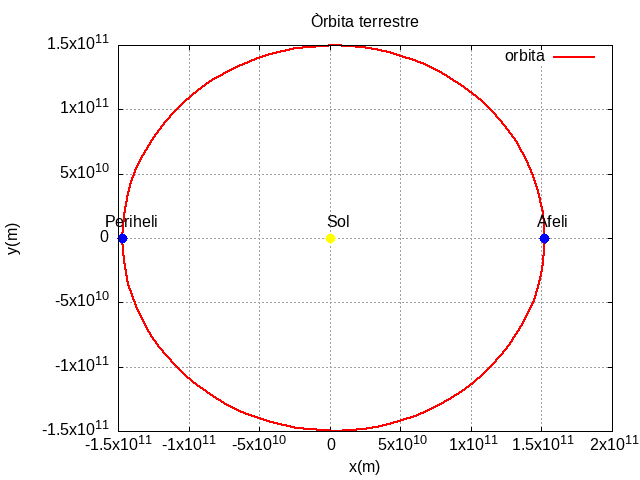
\includegraphics[width=\textwidth]{orbita.png}
        \caption{Òrbita Terrestre calculada numèricament amb el mètode d'Euler.}
        \label{fig: orb_terra}
    \end{subfigure}
    \hspace{0.1\textwidth}
    \begin{subfigure}{0.4\textwidth}
        \centering
        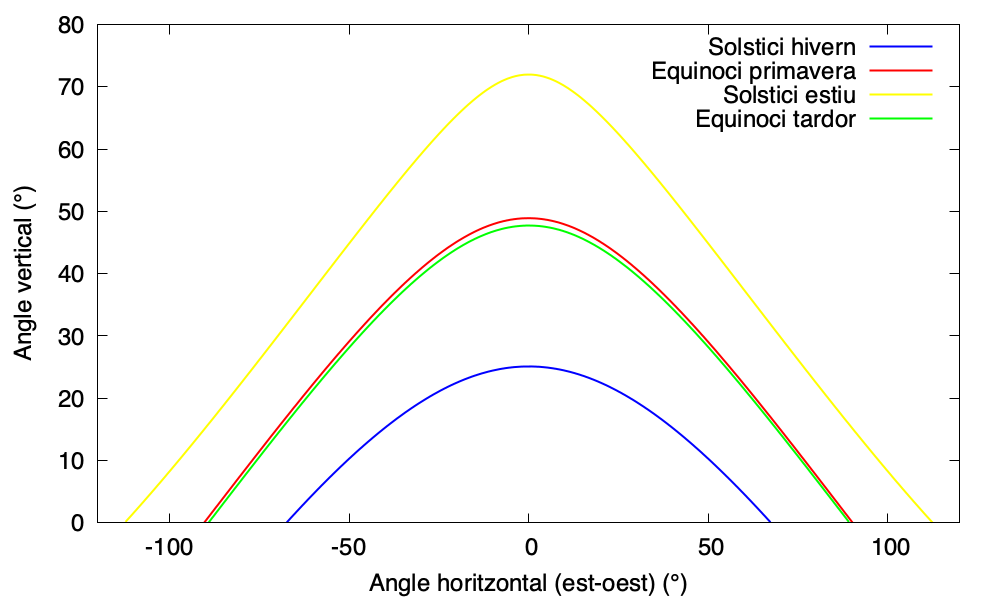
\includegraphics[width=\textwidth]{equinocis.png}
        \caption{Angles del Sol al llarg d'un dia per diferents moments de l'any a un habitatge de Sant Cugat del Vallès.}
        \label{fig: solsticis}
    \end{subfigure}
\caption{Resultats gràfics de les seccións \ref{sec: seccio_1} i \ref{sec: seccio_2}.}
\end{figure}

\section{Estudi energètic de la placa}
\subsection{Potència elèctrica produïda per un panell solar}
Suposant que el Sol és un cos negre esfèric a temperatura $T_S$ i de radi $R_S$, utilitzant la llei de Stefan-Boltzmann la potència que emet és $P_S=\sigma_{SB}T_S^44\pi R_S^2$. La intensitat de la radiació en un punt a una distància ${\rho}$ del Sol $I_{\rho}$ és igual la potència $P_S$ dividida entre l'àrea del front d'ona de la radiació, que és una closca esfèrica de radi ${\rho}$. Si el punt es troba a la superfície terrestre,  per l’efecte de l’albedo $\alpha_A$ cal multiplicar $I_{\rho}$ per $\alpha=1-\alpha_A$, la fracció de radiació absorbida per la Terra. Així doncs, la intensitat de la radiació incident és:
\begin{equation}
    I_{abs} = \alpha \frac{P_S}{4\pi \rho^2}=\alpha \frac{1}{\rho^2} R_S^2\sigma_{SB} T_S^4 \ .
    \label{I_abs}
\end{equation}
La intensitat efectiva que rebrà un panell solar és $I_{abs} \cos{\theta}$, on $\theta$ és l'angle entre la direcció de la llum incident i la normal al panell. Finalment, la potència elèctrica generada és igual al producte d'aquesta intensitat i l'àrea del panell, $A$, i un factor $r$, el seu rendiment. Així,
\begin{equation}
    P = r I_{abs} A \cos{\theta} = r \alpha \frac{1}{\rho^2}R_S^2\sigma_{SB}T_S^4A \cos{\theta} \ .
    \label{potencia placa}
\end{equation}
Els valors numèrics de $\alpha$, $R_S$, $\sigma_{SB}$ i $T_S$ els hem obtingut de les fonts \cite{Earth}, \cite{Sun} i \cite{Universe}.

A continuació normalitzem aquesta expressió. En quant a la variable $\theta$, al tractar-se d'un angle ja és adimensional, i per tant la donem per normalitzada. En quant a les altres dues variables,
\begin{align}
    \hat{P}=\frac{P}{P_0} \label{P normalizada} \\
    \hat{\rho}= \rho \left( r \alpha R_S^2\sigma_{SB}T_S^4A/P_0 \right)^{-1/2} \label{rho normalizada}
\end{align}
on hem escollit $P_0=400$ W per a normalitzar la potència. Segons l'enunciat, és la màxima electricitat que pot generar la placa i es produeix quan $I_0=10^3$ W/$\text{m}^2$ de radiació incideix sobre la mateixa. També utilitzem aquests valors per calcular el valor del rendiment $r$ de la placa de la següent manera:
\begin{equation}
     r = \frac{P_0}{I_0A} \ .
\end{equation}

Cal destacar que durant la pràctica fixem a 400 W la potència màxima que la placa pot generar.
Així doncs, segons aquesta normalització l'Eq. \eqref{potencia placa} esdevé:
\begin{equation}
    \hat{P} = \frac{\cos{\theta}}{\hat{\rho}^2} \ .
    \label{pot norm}
\end{equation}
Per a determinar $\cos{\theta}$, utilitzem la següent expressió:
\begin{equation}
    \cos \theta = \cos \theta_z \cos \beta + \sin \theta_z \sin \beta \cos (\eta - \gamma) \ .
    \label{cos theta}
\end{equation}
amb $\theta_z = 90^{\circ}-\nu$, on els angles $\eta$ i $\nu$ ja han estat definits i calculats a la secció anterior, i són les variables que determinen $\theta$. Els angles $\beta$ i $\gamma$ són paràmetres que fan referència a la inclinació i orientació de la placa; es defineixen formalment a la secció \ref{sec: demo cos theta} de l'Annex, on es demostra l'equació.

En la Fig. \ref{fig: potencia}, es representa la potència produïda pel panell al llarg d'un cert dia.

\begin{figure}[H]
    \centering
    \begin{subfigure}{0.5\textwidth}
        \centering
        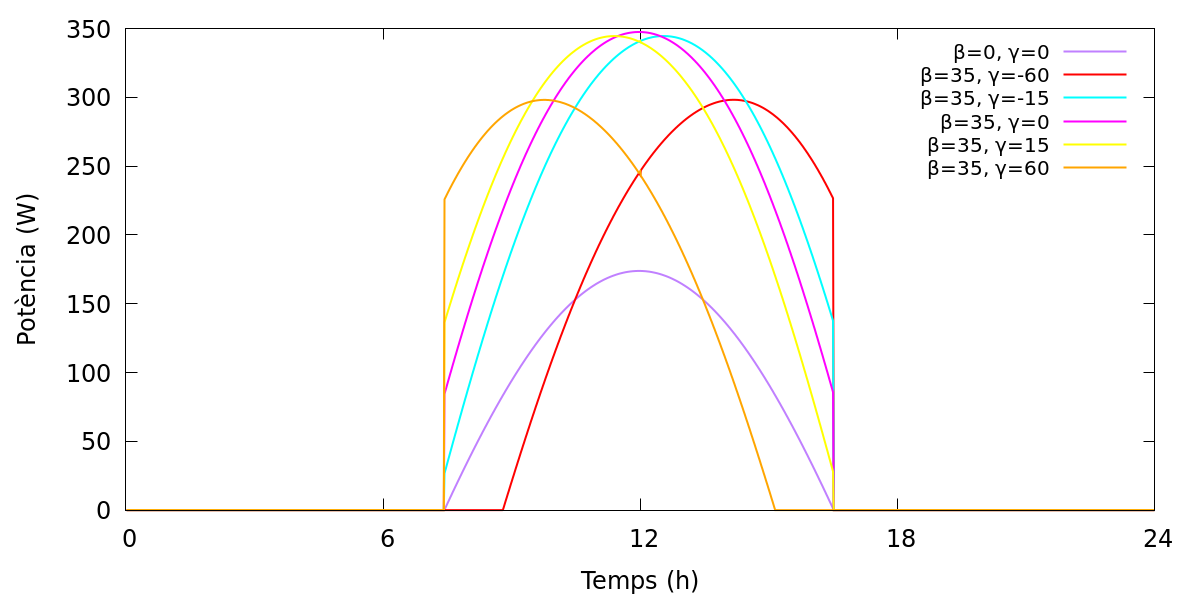
\includegraphics[width=\textwidth]{dia_3gener_pot_plot.png}
        \caption{Potència elèctrica produïda per la placa durant el dia 3 de gener.}
        \label{fig: potencia}
    \end{subfigure}%
    \hspace{0.000001\textwidth}%
    \begin{subfigure}{0.5\textwidth}
        \centering
        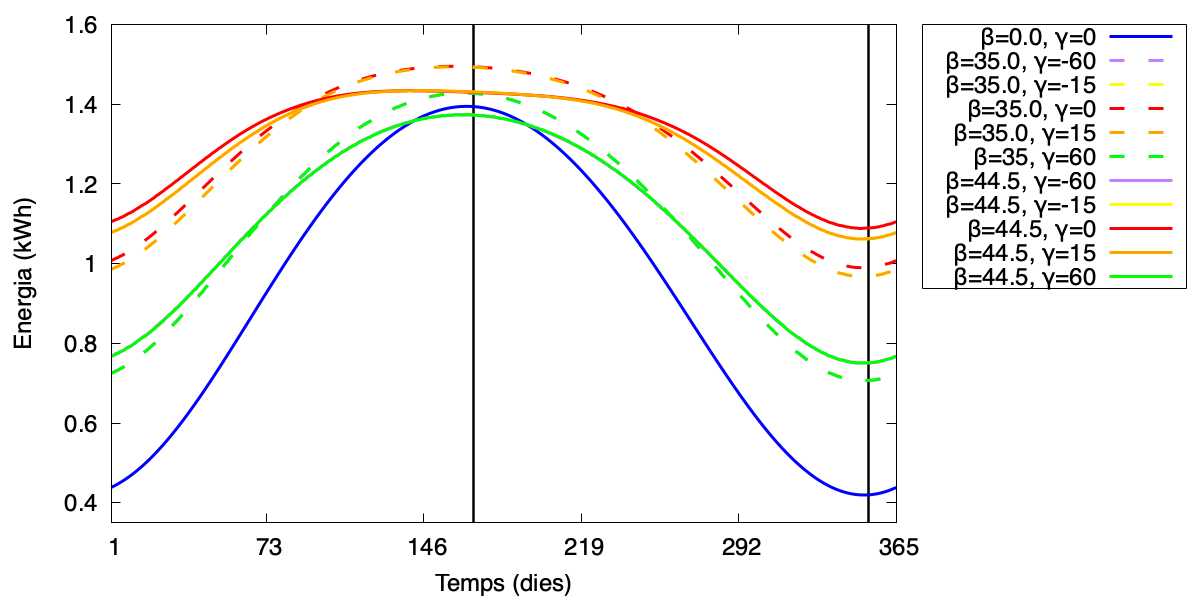
\includegraphics[width=\textwidth]{energia.png}
        \caption{Energia elèctrica produïda per la placa cada dia de l'any.}
        \label{fig: energia}
    \end{subfigure}
    \caption{Gràfics referents a l'estudi energètic de la placa.}
    \label{estudi energia}
\end{figure}

Quan $\beta=0^{\circ}$, es representa la gràfica per un sol valor de $\gamma$ (escollim arbitràriament $\gamma=0^{\circ}$) perquè el terme $\sin\beta$ en l’Eq. \eqref{cos theta} s’anul·la, i per tant desapareix la dependència en $\gamma$.

Si $\theta_z$ o $\theta$ surten del rang $[-\pi/2,\pi/2]$ hem imposat que la potència sigui nul·la. Quan $\theta_z \notin [-\pi/2,\pi/2]$, el Sol es troba per sota de l'horitzó, impedint que arribi llum a la placa. És per això que mentre que per $\beta = 0^{\circ}$ la potència s'anul·la gradualment, per $\beta \neq 0^{\circ}$ s'anul·la bruscament, ja que quan el Sol és a prop de l’horitzó $\theta$ encara és inferior a $90^{\circ}$. Similarment, quan $\theta \notin [-\pi/2,\pi/2]$ el Sol està situat darrere la placa, sent ella mateixa la que bloqueja la llum. És per això que quan $\gamma$ és prou gran, com ara en la Fig. \ref{fig: potencia} per $\gamma=\pm60^{\circ}$, la potència s'anul·la abans que el Sol estigui a l'horitzó. A la secció \ref{sec: dia estiu potencia} de l'Annex, es comparen aquests resultats amb els obtinguts en un dia d'estiu.

\subsection{Energia elèctrica produïda per un panell solar}
Amb la potència elèctrica generada per la placa cada minut de l'any ens disposem a calcular l'energia elèctrica produïda per aquesta. La potència és la derivada temporal de l'energia, per tant, podem trobar l'energia elèctrica produïda per la placa durant una certa quantitat de temps integrant numèricament la potència respecte el temps. Per fer-ho, hem optat pel mètode d'integració numèrica de Simpson $\frac{1}{3}$. Presentem l'energia produïda cada dia de l'any per diferents combinacions dels angles $\beta$ (inclinació i orientació de la placa) i $\gamma$ (orientació de la placa) a la Fig. \ref{fig: energia}.


%\begin{figure}[H]
    %\centering
    %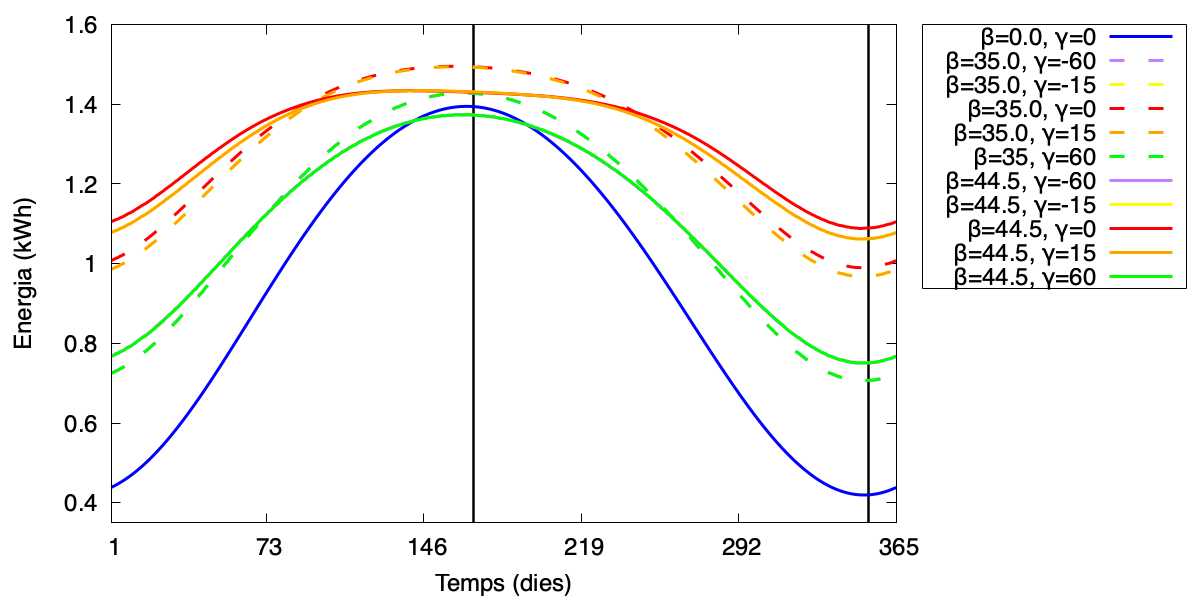
\includegraphics[width=0.75\linewidth]{energia.png}
    %\caption{Energia elèctrica produïda per la placa cada dia de l'any.}
    %\label{fig: energies}
%\end{figure}

Les linies negres verticals indiquen els solsticis d'estiu i d'hivern per a una millor interpretació dels resultats. A més, podem veure com per a una $\gamma$ donada, en el gràfic no s'aconsegueix distingir entre el perfil corresponent al valor positiu o negatiu de la mateixa, ja que són pràcticament iguals.

Pel que fa a la normalització del problema numèric, ens ha quedat la següent equació normalitzada.
\begin{equation}
    \hat{E} = \int \hat{P} \, d\hat{t}
    \label{energia}
\end{equation}
on $\hat{t}=\frac{t}{t_0}$, $\hat{P}=\frac{P}{P_0}$ i $\hat{E}=\frac{E}{P_0 t_0}$, amb $t_0=86400$ s (els segons que hi ha en un dia) i $P_0=400$ W (la potència màxima de la placa en les condicions donades a l'enunciat de la pràctica). 
\subsection{Extra: Optimització dels angles de la placa}

Hem plantejat el problema des del punt de vista de maximitzar la producció d'energia total al llarg d'un any mantenint els angles $\beta$ i $\gamma$ de la placa constants durant tot l'any. Per fer-ho, hem utilitzat que si tenim en compte l'Eq. \ref{potencia placa} i \ref{cos theta}, l'energia total normalitzada produïda en un any la podem escriure com
\[
\hat{E}_T(\beta, \gamma) = \cos \beta \int \hat{P}_{opt} \cos \theta_{z} \, d\hat{t} + \sin \beta \cos \gamma \int \hat{P}_{opt} \sin \theta_{z} \cos \eta \, d\hat{t} + \sin \beta \sin \gamma \int \hat{P}_{opt} \sin \theta_{z} \sin \eta \, d\hat{t} \equiv
\]
\[
\equiv \hat{a}\cos \beta
+ \hat{b}\sin \beta \cos \gamma
+ \hat{c}\sin \beta \sin \gamma
\]
on $\hat{P}_{opt}=\frac{r I_{abs} A}{P_0}$, $\hat{t}=\frac{t}{t_0}$ i $\hat{E}=E P_0 t_0$

Igualant el gradent a 0, trobem que
\[
\left.
\begin{aligned}
-\hat{a}\sin \beta + \hat{b}\cos \beta \cos \gamma + \hat{c}\cos \beta \sin \gamma = 0 \\
-\hat{b}\sin \beta \sin \gamma + \hat{a}\sin \beta \cos \gamma = 0
\end{aligned}
\right\}
\]
La solució corresponent per $\beta$ i $\gamma$ és
\[
\gamma = \arctan\left(\frac{\hat{c}}{\hat{b}}\right), \quad \beta = \arctan\left(\frac{\hat{b} \cos(\gamma) + \hat{c} \sin(\gamma)}{\hat{a}}\right)
\]
on hem descartat la solució corresponent a $\beta=n\pi$ per no ser un màxim.

Calculant numèricament les integrals $\hat{a}$, $\hat{b}$ i $\hat{c}$ per Simpson 1/3 sota la condició de que $-\frac{\pi}{2} \leq \theta_z \leq \frac{\pi}{2}$ (en cas contrari l'integrand l'hem anul·lat), hem obtingut uns angles òptims arrodonint a la primera xifra decimal de $\gamma=0^\circ$ i $\beta=44,5^\circ$. L'energia produïda dia a dia durant tot l'any corresponent a aquests angles pot trobar-se a la Fig. \ref{fig: energia}. 

A la Fig. \ref{fig: energies} podem observar que a l'estiu un angle d'inclinació de $35^\circ$, per exemple, produeix més energia que un de $44,5^\circ$, ara bé, com hem dit, nosaltres hem maximitzat la producció total durant l'any. Això, però, suggereix que durant diferents èpoques de l'any podriem modificar la inclinació de la placa per així maximitzar la seva producció en cada període i conseqüentment durant tot l'any.

\section{Resolució de l'EDO per diversos mètodes numèrics}\label{sec: edos}
Per a resoldre l'EDO de l'òrbita terrestre hem utilitzat el mètode d'Euler, però sabem que hi ha mètodes numèrics més potents que aquest. Per axò hem volgut comparar els resultats.

Els mètodes emprats per a resoldre l'equació \eqref{equ_en_r} han estat el Runge-Kutta d'ordre 2 i el Runge-Kutta d'ordre 4\footnote{els seus corresponents gràfics i errors relatius pel que fa al radi orbital es troben a l'annex \ref{sec: orbitesRK}}, amb la mateixa discretització temporal en els 3 mètodes numèrics.

\begin{figure}[H]
    \centering
    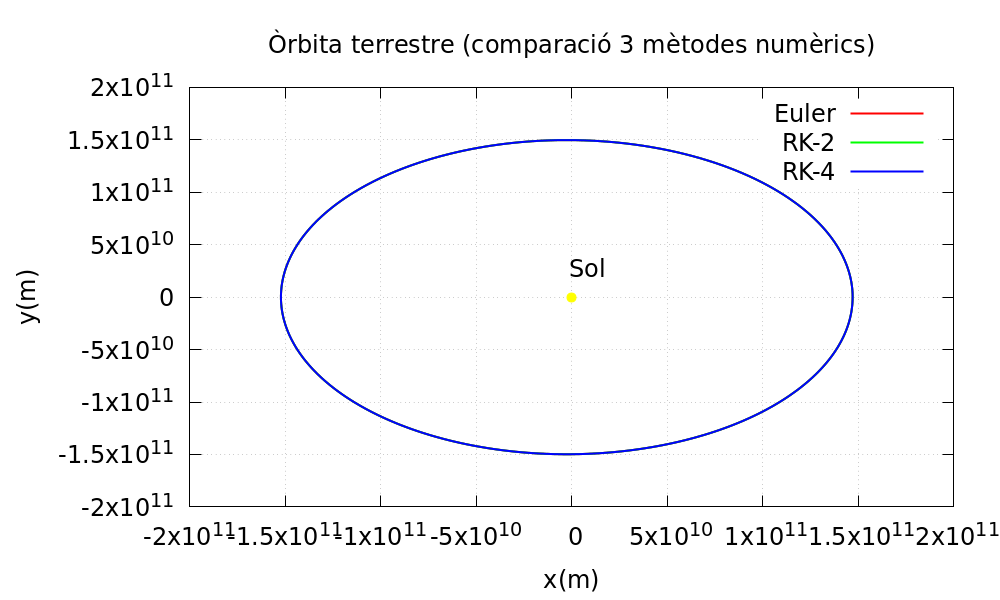
\includegraphics[width=0.4\textwidth]{orbita3met.PNG}
    \caption{Comparació òrbita terrestra per 3 mètodes numèrics}
    \label{fig: orbita3met}
\end{figure}

Observant els gràfics \ref{fig: orbita3met} podem veure que les diferències entre les òrbites càlculades pels diferents mètodes numèrics són realment mínimes.

\section{Consideració de la Terra com no esfèrica}\label{sec: terranoesfera}
Fins ara hem estat considerant que la Terra tenia forma d'una esfera perfecta. Però sabem que realment, la força centrífuga generada per la seva pròpia rotació provoca una deformació en els pols, 'aixafant-la' i fent que la Terra no sigui una esfera.

Això no ens afecta al càlcul de l'òrbita terrestre ja que aquesta només considera la distància del sol al centre de la Terra però sí afecta en la resta de càlculs ja que el Radi de la Terra deixa de ser constant. En aquest apartat, aproximarem la Terra a un esferoide, com a un el·lipsoide de revolució. Podem arribar a les següents expressions\footnote{El procés per arribar a aquestes equacions està descrit en l'annex \ref{sec: terraesferoidedibuix}}:

\begin{equation}
    tan(\alpha_{T_{el}}) = \frac{b}{a}tan(\alpha) 
    \label{eq: alphatel}
\end{equation}

\begin{equation}
    r_{T_{el}} = \sqrt{\frac{(a^2cos(\alpha_{T_{el}})^2+(b^2sin(\alpha_{T_{el}}))^2}{(acos(\alpha_{T_{el}}))^2+(bsin(\alpha_{T_{el}}))^2}}
    \label{eq: rtel}
\end{equation}

Aquestes ens permeten calcular el Radi de la nostra esferoide (distància superfície-centre terreste) en funció de l'angle de latitud $\alpha$, calculat ja a partir de la dades geogràfiques en la secció \ref{sec: seccio_2}. Redefinim $r_T$ com $r_{T_el}$ i $\alpha$ com $\alpha_{T_{el}}$ per poder calcular el nou vector $\vec{r_{(t)}}$ amb l'equació \eqref{vector_r}. Els passos per a la simulació són exactament els mateixos que els ja definits a les corresponents seccions \ref{sec: seccio_2}.

\section{Conclusions}
En aquesta pràctica hem estudiat l'energia elèctrica produïda per una instal·lació de panells solars fotovoltaics a Catalunya. Amb les dues primeres seccions hem simulat la posició del Sol respecte la posició de la placa. Considerant el Sol com un cos fix generador de camp gravitatori i la Terra com l'únic objecte astronòmic existent hem obtingut un error acumulat en el radi de l'òrbita al cap d'un any de menys del $0,00001\%$. Concretament, al primer apartat hem resolt numèricament l'equació del moviment de la Terra amb el mètode d'Euler i al segon apartat hem calculat geomètricament la posició del Sol al cel des d'un habitatge de Catalunya. Amb les dades aconseguides a aquests apartats, a la tercera secció ens hem volcat a l'estudi de l'energia produïda pels panells solars tot aproximant el Sol com un cos negra esfèric. En aquest apartat hem obingut una energia mitjana produïda al dia de [???], dada molt semblant a la proporcionada per la [xxxxxx] i que valida el nostre model.

A més, s'ha trobat en quina posició (descrita pels angles òptims) ha d'estar la placa per a produir el màxim d'energia elèctrica, la qual s'ha considerat pel període de temps d'un any. Per últim, al repetir les simulacions amb altres models que consideressin aproximacions que ens apropéssin cada cop més a la realitat per posteriorment comparar els resultats. Concretament hem escollit calcular l'òrbita Terrestre al voltant del sol amb altres mètodes numèrics: Runge-Kutta d'ordre 2 i Runge-Kutta d'ordre 4, emprant la mateixa discretització del temps que per Euler. Per altra banda també hem canviat el model aproximat al considerar la Terra (fins ara pensada com una esfera) com a un esferoide. Cap d'aquests canvis ha sigut molt significatiu en els resultats obtinguts d'aquestes noves simulacions. 

\section*{Annex}
\appendix

\section{Link al repositori}
\vspace{-1em}
A continuació donem el link per a accedir al repositori de github on es troba el codi: \href{https://github.com/isaacbg25/Sol/tree/main}{link}


\section{Deducció de les equacions de moviment de l'òrbita terrestre}
\label{annex: equ_mov}


Per aquest tipus de sistemes i considerant únicament la força central definida a l'Eq. \eqref{si}, podem definir dues equacions de moviment en el pla polar 
\begin{equation}
    F(r)=m\ddot{r}-mr{\dot{\theta}}^2
    \label{equ_en_r}
\end{equation}
\begin{equation}
    0=\ddot{\theta}m=mr\ddot{\theta}+2m\dot{r}\dot{\theta}
    \label{equ_en_theta}
\end{equation}
Si, a més, tenim en compte la conservació del moment angular, podem escriure
\begin{equation}
    L=mr\dot{\theta}=ctt
    \label{moment_angular}
\end{equation}
Combinant les Eq. \eqref{equ_en_r} i \eqref{moment_angular} obtenim una EDO que només depen de r i una altra que només depen de $\theta$
\begin{equation}
    \frac{\partial\dot{r}}{\partial t}=-GM\frac{1}{r^2}+\frac{L^2}{m^2r^3}
    \label{edor}
\end{equation}
\begin{equation}
    \frac{\partial\theta}{\partial t}=\frac{L}{mr^2}
    \label{edot}
\end{equation}
Normalitzant aquestes dues equacions i reduint l'ordre de l'Eq. \eqref{edor}, obtenim
\begin{equation}
    \frac{\partial\tilde{v}}{\partial\tilde{t}}=-\frac{1}{\tilde{r}^2}+\frac{1}{\tilde{r}^3}, \quad
    \frac{\partial\tilde{r}}{\partial\tilde{t}}=\tilde{v}, \quad
    \frac{\partial\tilde{\theta}}{\partial\tilde{t}}=\frac{1}{\tilde{r}^2}
    \label{eq:all}
\end{equation}
on les variables normalitzades segueixen $r=\tilde{r}\alpha$, $t=\tilde{t}\frac{\alpha}{\bar{v}}$ i $v=\tilde{v}\bar{v}$ i les constants de normalització $\alpha = \frac{\beta}{\kappa}$, $\bar{v}=\frac{\kappa}{(\beta)^{1/2}}$, $\beta=\frac{L^2}{m^2}$ i $\kappa=GM$.


\section{Matrius de canvi de sistema de referència}\label{annex: matr_rot}
\begin{equation}
    \mathbf{R}_{\beta}=
    \begin{pmatrix}
      1 & 0 & 0   \\
      0 & \cos\beta& -sin\beta \\
      0 & sin\beta & cos\beta \\
    \end{pmatrix}
\end{equation}  

\begin{equation}
    \mathbf{R}_{\gamma}=
    \begin{pmatrix}
       \cos\beta& -sin\beta& 0 \\
       \sin\beta & cos\beta &0\\
      0 & 0 & 1  \\
    \end{pmatrix}
\end{equation}  


\section{Angles i vectors apartat 2}
\begin{figure}[hbt]
    \centering
    \begin{subfigure}{0.5\textwidth}
        \centering
        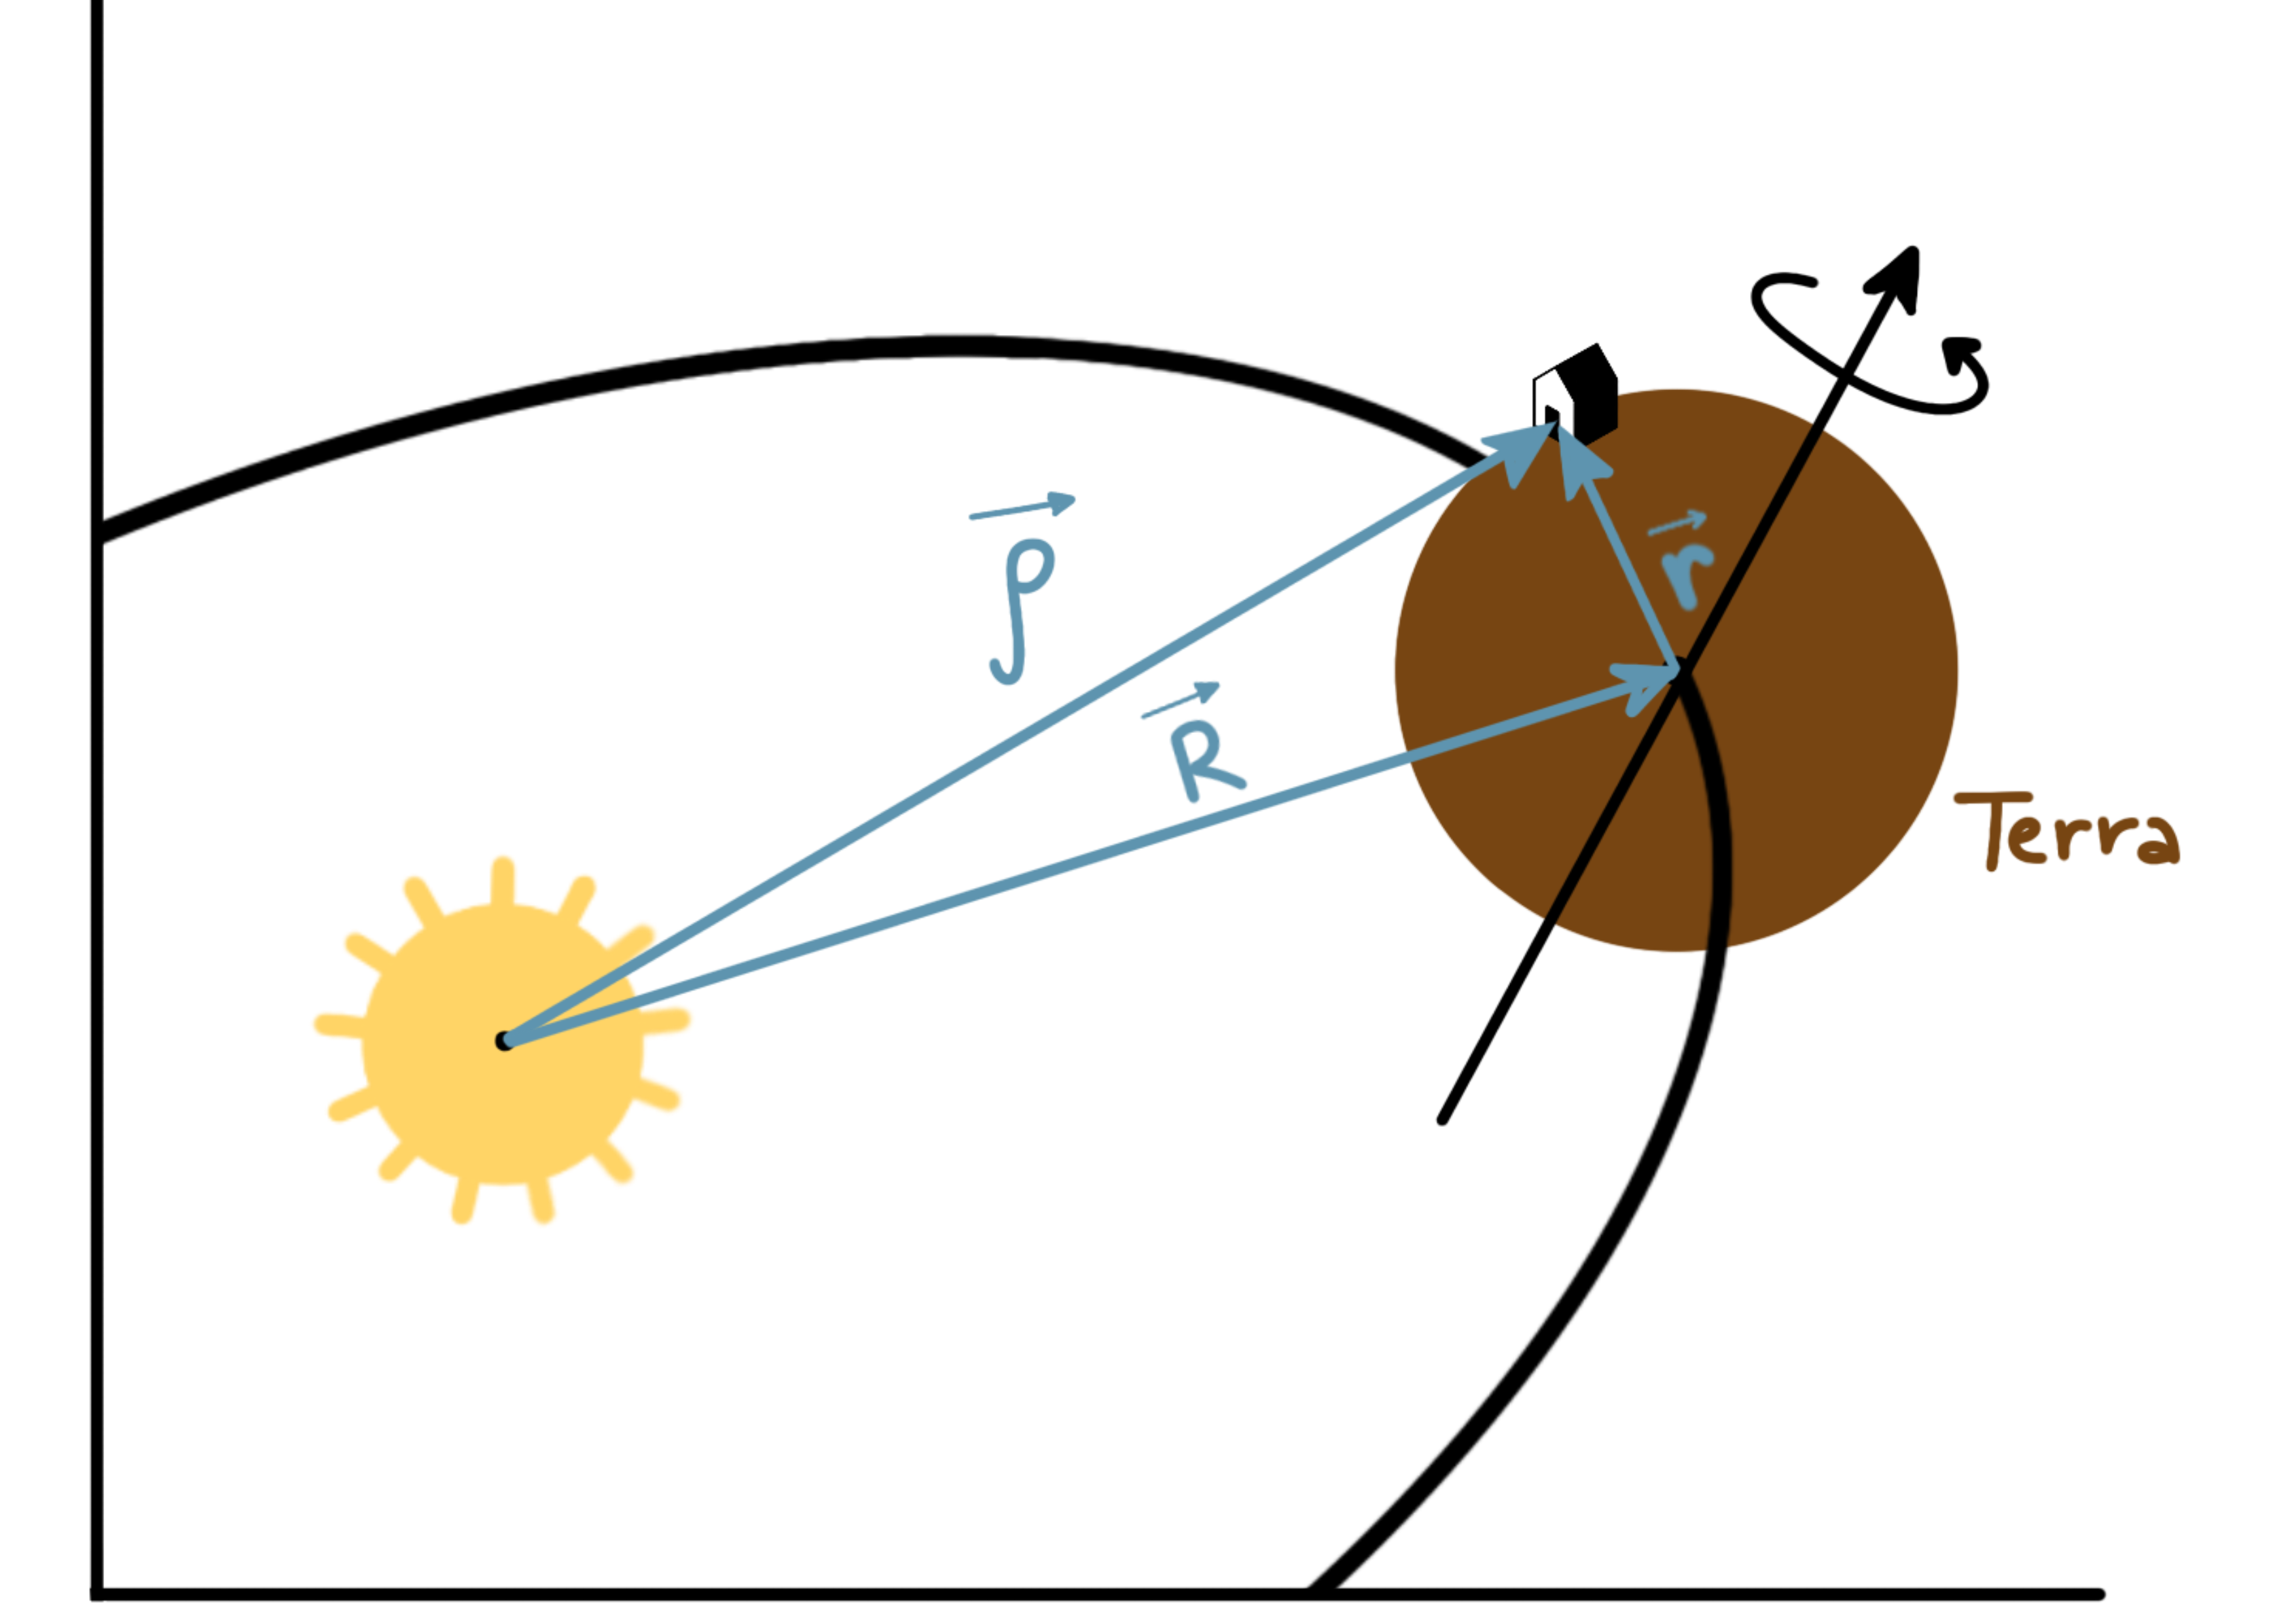
\includegraphics[width=\textwidth]{vectors.PNG}
        \caption{Els vectors que hem definit per determinar els angles de la posició del Sol.}
        \label{fig: sist_vectors}
    \end{subfigure}%
    \hspace{0.000001\textwidth}%
    \begin{subfigure}{0.5\textwidth}
        \centering
        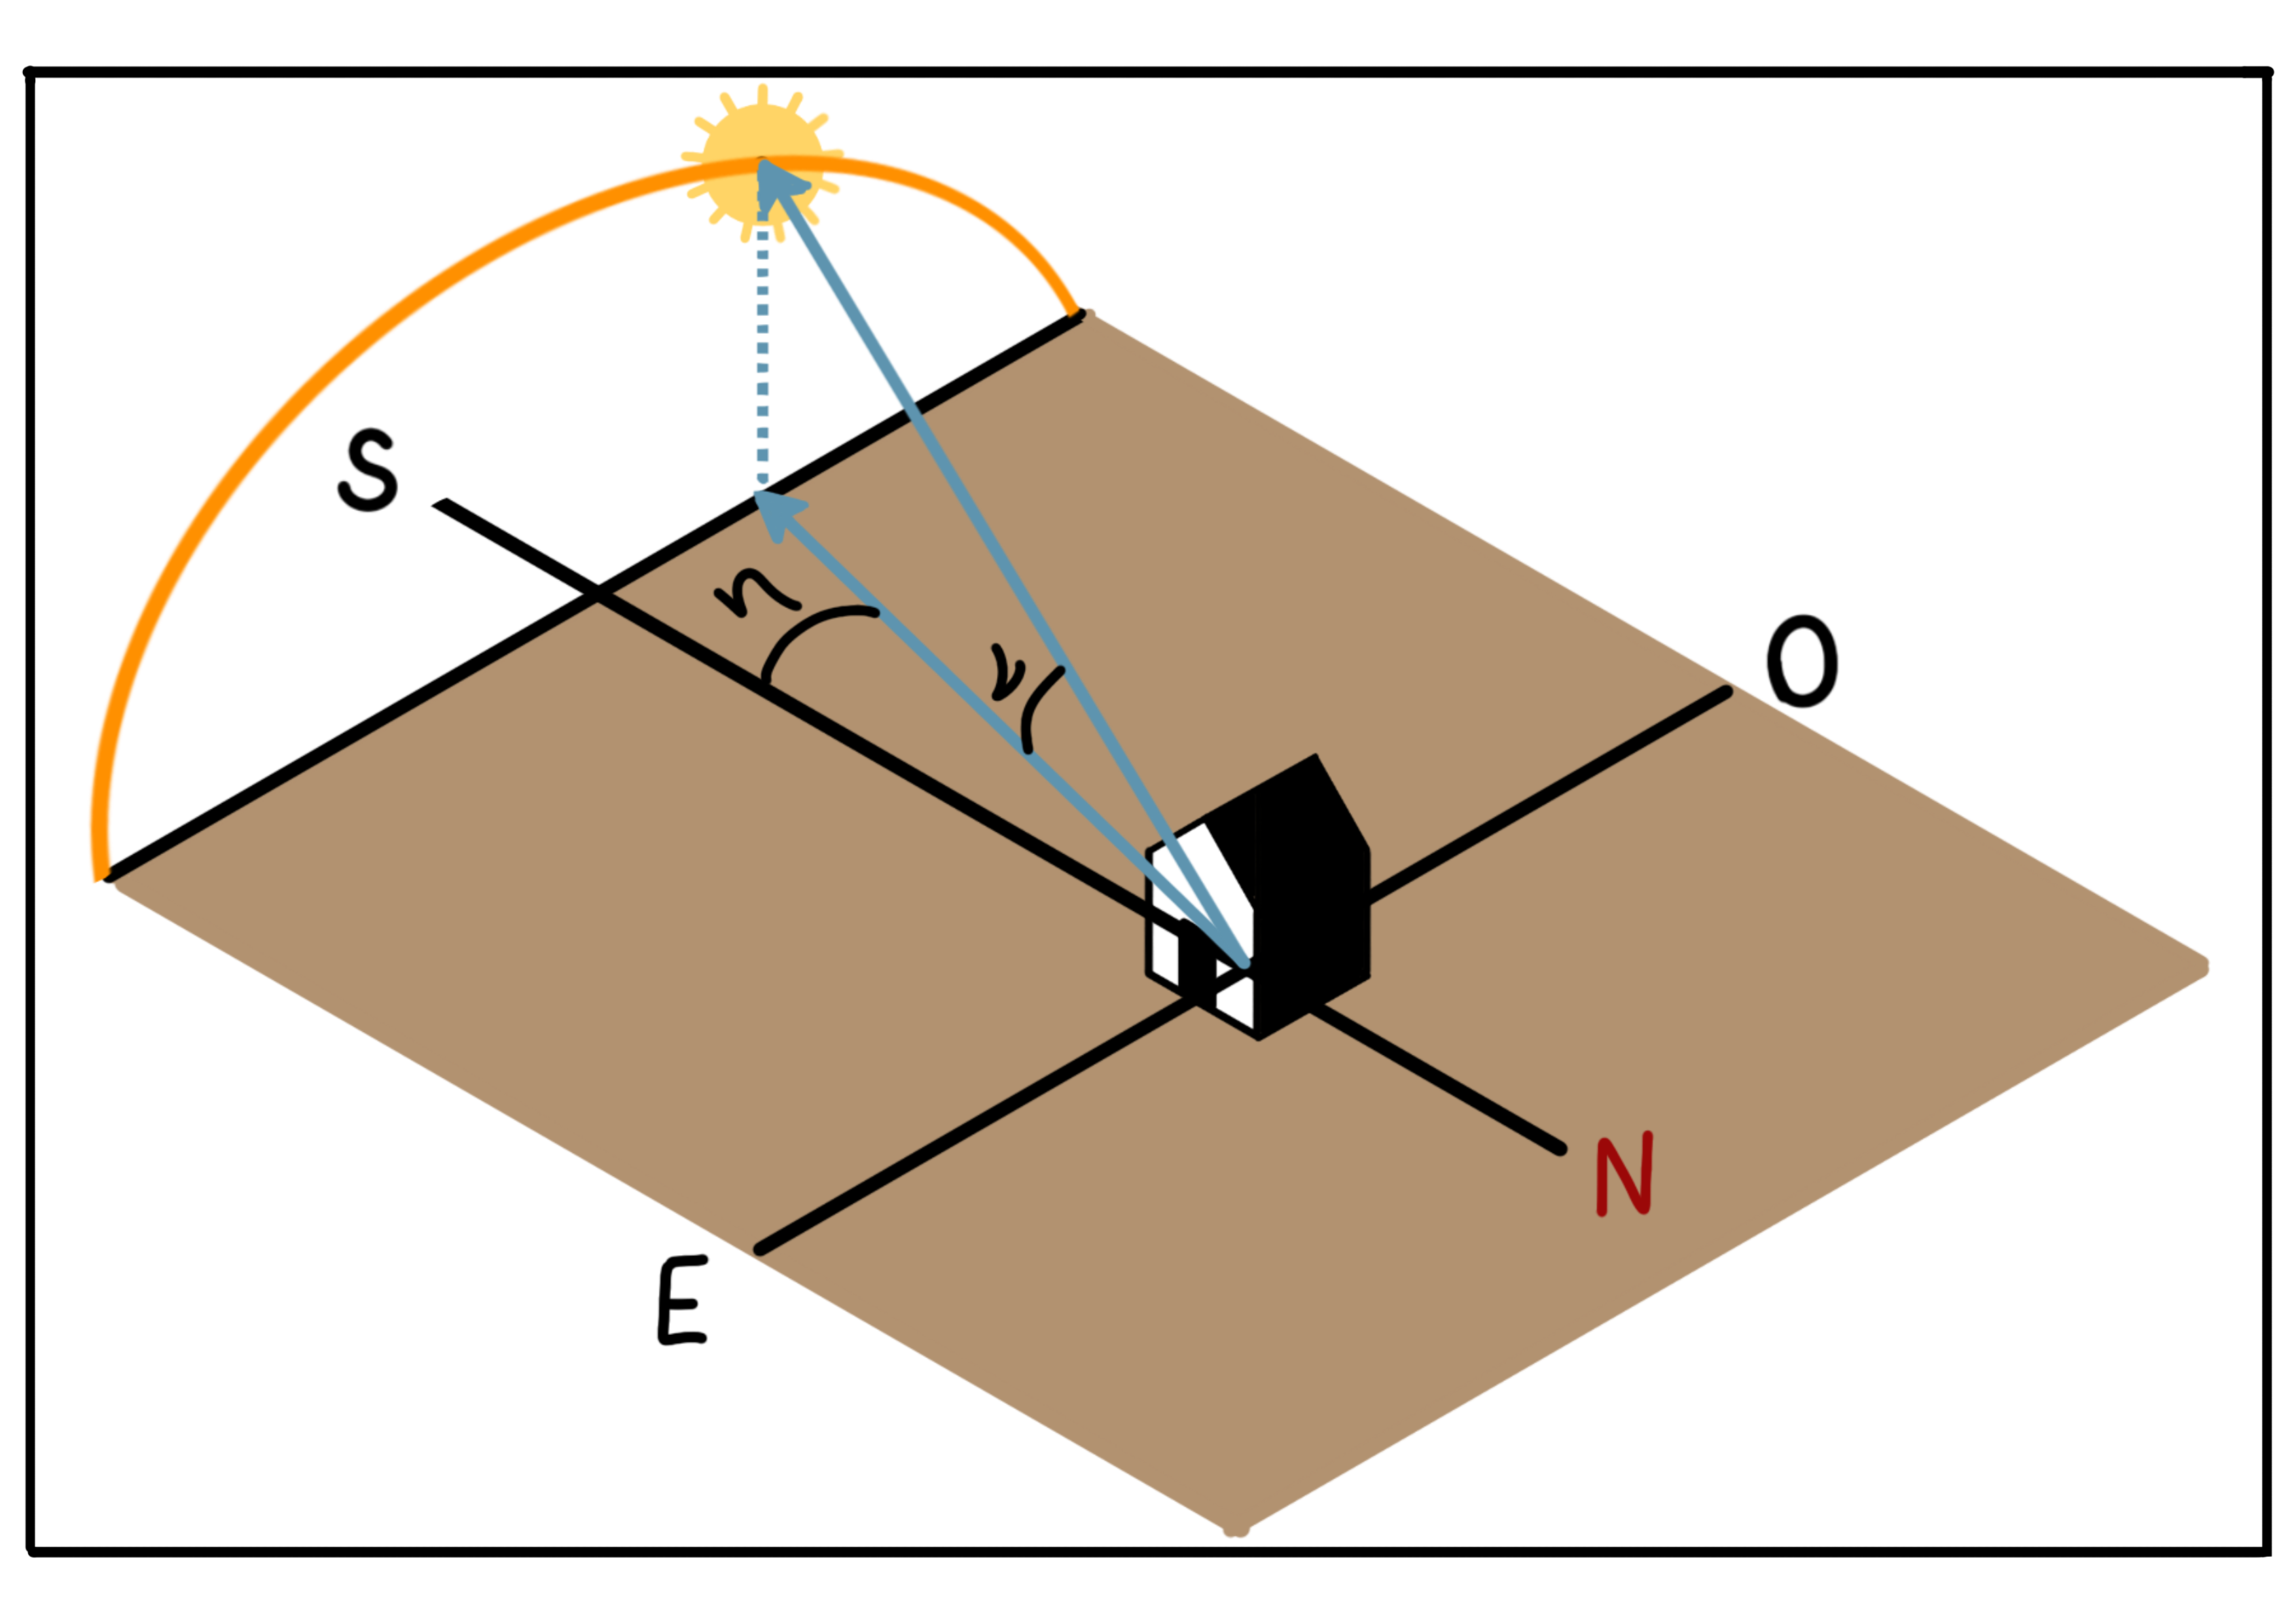
\includegraphics[width=\textwidth]{ang_sol.PNG}
        \caption{Els dos angles que hem usat per a determinar la posició del Sol.}
        \label{fig: sist_sol}
    \end{subfigure}
\label{fig: sistemes1}
\caption{Vectors i angles definits a la seccio \ref{sec: seccio_2}.}
\end{figure}

\begin{figure}[hbt]
    \centering
    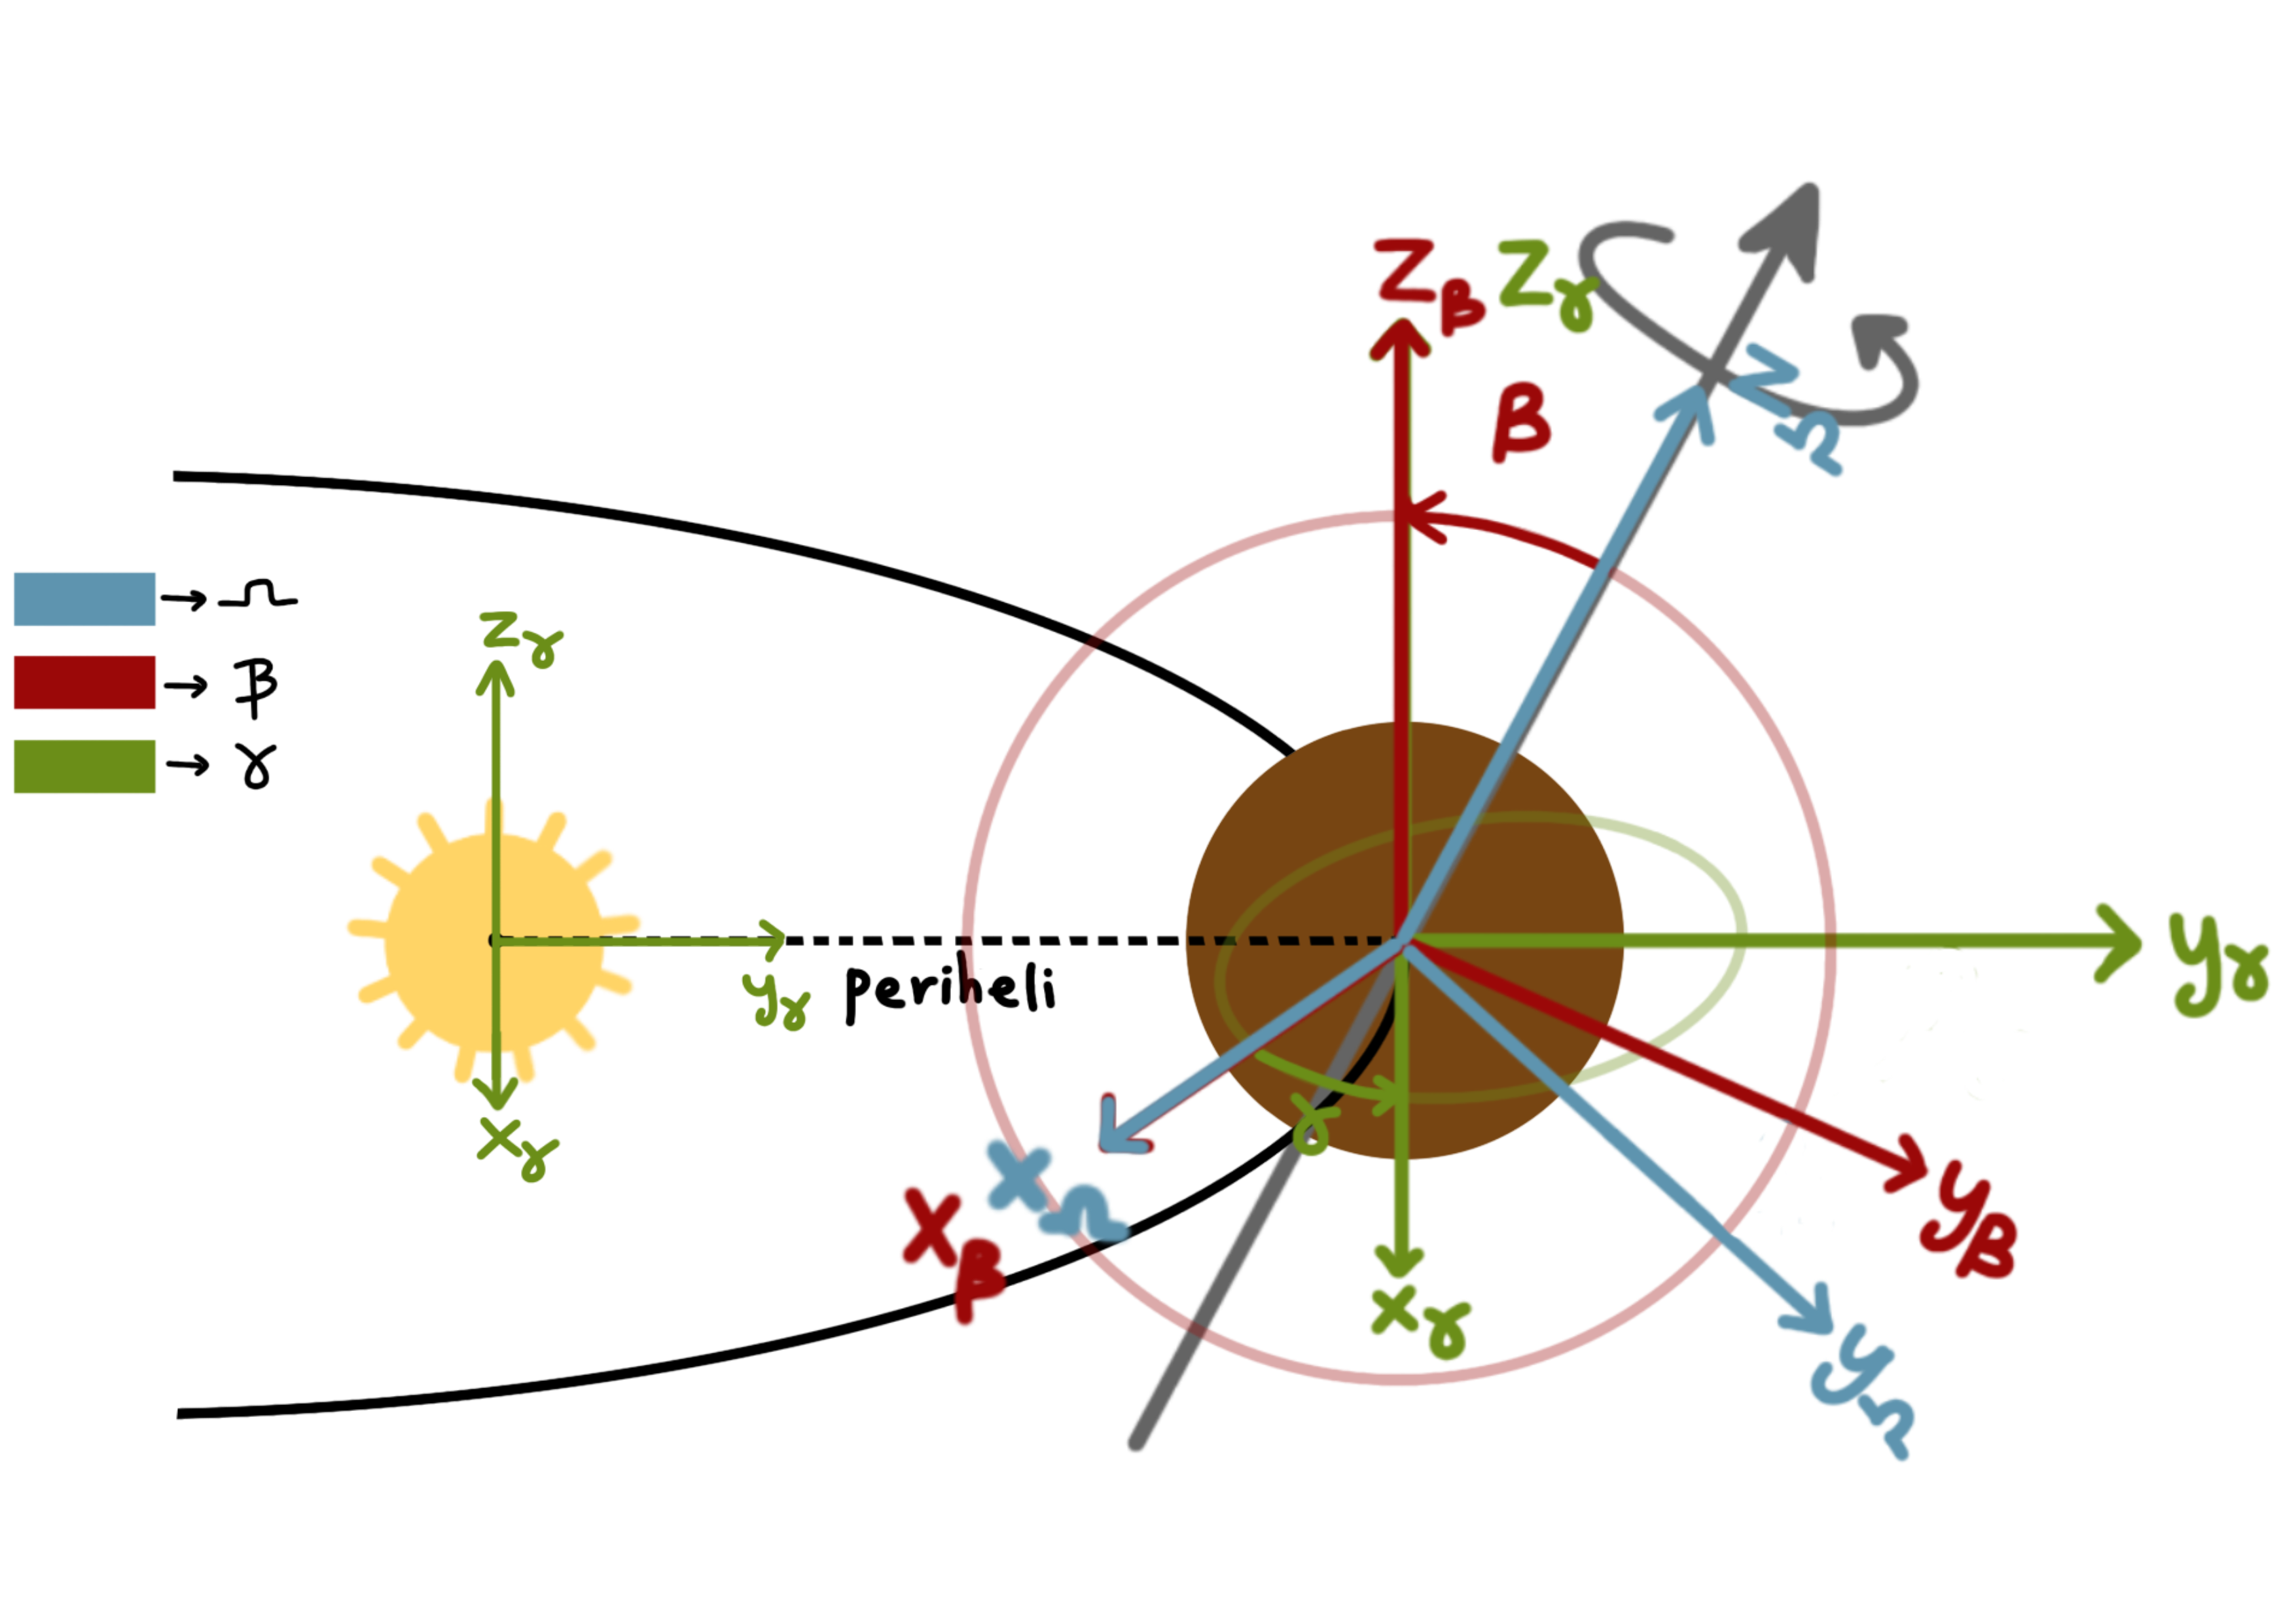
\includegraphics[width=0.5\textwidth]{sist_ref.PNG}
    \caption{Diferents sistemes de referència de la secció \ref{sec: seccio_2}.}
    \label{fig: sist_ref}
\end{figure}

\section{Demostració de l'Eq. \eqref{cos theta}}
\label{sec: demo cos theta}
En aquesta secció demostrarem l'Eq. \eqref{cos theta}

Els angles $\theta$, $\theta_z$, $\nu$ i $\eta$ ja han estat definits en anteriors apartats. En quant els angles $\beta$ i $\gamma$, donem les seves definicions formalment a continuació.
\begin{itemize}
    \item $\beta$, Angle zenital de la placa (inclinació o pendent): l'angle que formen el pla del panell i l'horitzontal; $0^\circ \leq \beta \leq 180^\circ$.
    \item $\gamma$, Angle azimutal de la placa (orientació): la desviació de la projecció sobre un pla horitzontal de la normal a la superfície respecte el meridià local; $-180^\circ \leq \gamma \leq 180^\circ$, i prenem el mateix conveni de signes que per $\eta$.
\end{itemize}

El vector unitari que apunta en la direcció del Sol amb origen al panell ve definit per:
\begin{equation}
    \mathbf{S} = (\sin \theta_z \cos \eta, \sin \theta_z \sin \eta, \cos \theta_z)
    \label{vector unitari sol}
\end{equation}
D'altra banda, el vector unitari que defineix la direcció normal a la superfície de la placa és:
\begin{equation}
       \mathbf{N} = (\sin \beta \cos \gamma, \sin \beta \sin \gamma, \cos \beta)
       \label{vector unitari placa}
\end{equation}
L'angle d'incidència de la radiació (\(\theta\)) és l'angle que formen el vectors \(\mathbf{S}\) i \(\mathbf{N}\), per definició. Per tant, tenint en compte que aquests vectors són unitaris:
\begin{equation}
    \cos \theta = \mathbf{S} \cdot \mathbf{N}
\end{equation}
Substituint els vectors per l'Eq. \eqref{vector unitari sol} i l'Eq. \eqref{vector unitari placa}, i operant:
\begin{align*}
    \cos \theta &= (\sin \theta_z \cos \eta, \sin \theta_z \sin \eta, \cos \theta_z) \cdot (\sin \beta \cos \gamma, \sin \beta \sin \gamma, \cos \beta) \\
    &= (\sin \theta_z \cos \eta)(\sin \beta \cos \gamma) + (\sin \theta_z \sin \eta)(\sin \beta \sin \gamma) + (\cos \theta_z)(\cos \beta) \\
    &= \sin \theta_z \sin \beta (\cos \eta \cos \gamma + \sin \eta \sin \gamma) + \cos \theta_z \cos \beta \\
    &= \cos \theta_z \cos \beta + \sin \theta_z \sin \beta \cos (\eta - \gamma)
\end{align*}

on a l'última igualtat hem aplicat la fórmula del cosinus de la diferència:
\[
\cos (\eta - \gamma) = \cos \eta \cos \gamma + \sin \eta \sin \gamma
\]

Això completa la demostració.


\section{Estudi de la potència en un dia d'estiu}
\label{sec: dia estiu potencia}

En la Fig. \ref{fig: potencia} com més proper és el valor de $\gamma$ a 0$^{\circ}$, major és el valor màxim de la potència. D'altra banda, per un determinat $\gamma$, la menor potència màxima assolida és per $\beta=0^{\circ}$. En el cas de la potència en un dia d'estiu, representat a la Fig. \ref{potencia dia estiu}, la potència màxima quan $\beta=0^{\circ}$ és notablement superior a la del 3 de gener. D'altra banda, en la gràfica per $\beta=35^{\circ}$ al migdia s'observa una disminució en la potència. A més, en tots els casos la duració del període de temps de generació de potència és superior a la del 3 de gener. Tot això es deu a que el dia és d'estiu. Per tant, la posició del Sol és més alta de manera que quan està al voltant de la seva alçada màxima l’angle $\theta$ és major per $\beta=0^{\circ}$, i disminueix amb la inclinació de la placa.


\begin{figure}[H]
    \centering
        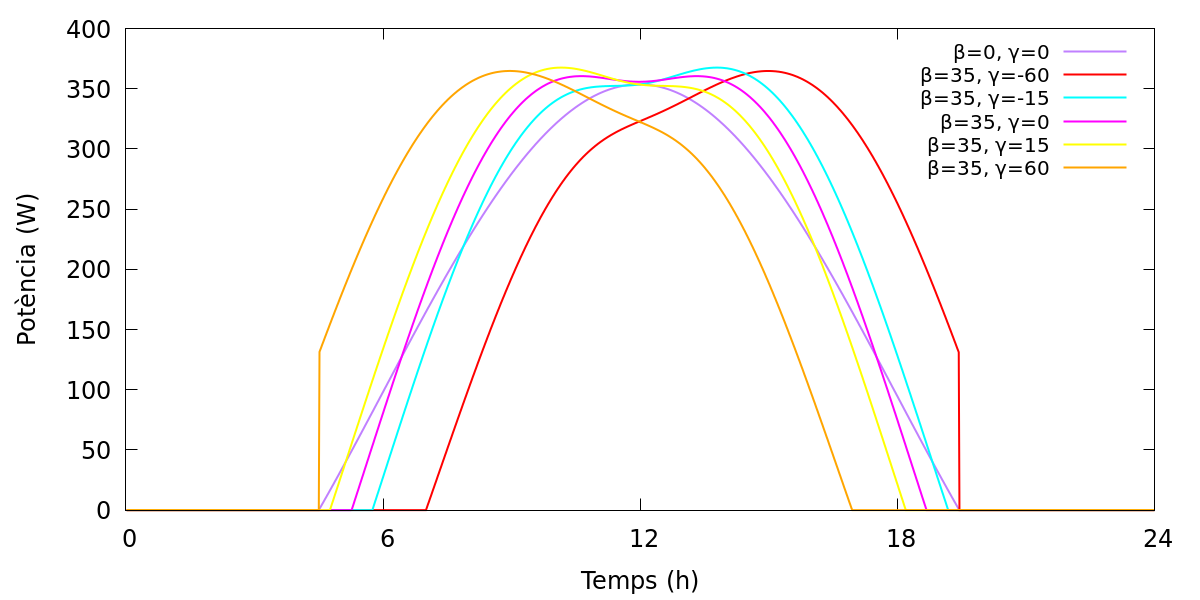
\includegraphics[width=\textwidth]{dia_estiu_pot_plot.png}
        \caption{Dia 170.}
        \label{fig: potencia dia 170}
    \caption{Potència elèctrica produïda per la placa durant un dia d'estiu per diversos valors de $\beta$ i de $\gamma$.}
    \label{potencia dia estiu}
\end{figure}

\section{Representació gràfica de les òrbites terrestres resultants}
\label{sec: orbitesRK}
\begin{figure}[H]
    \centering
    \begin{subfigure}{0.5\textwidth}
        \centering
        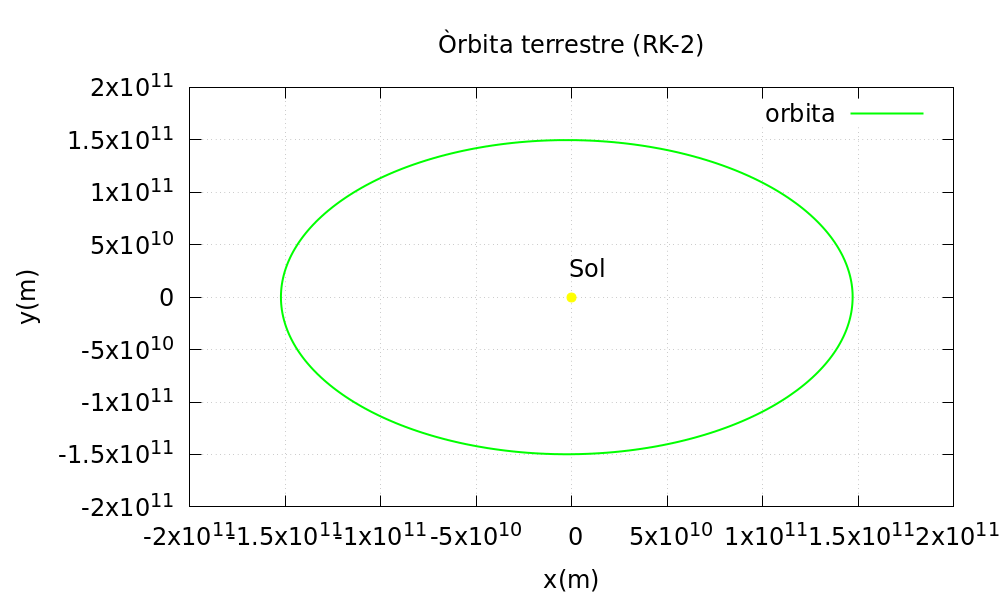
\includegraphics[width=\textwidth]{orbitaRK2.PNG}
        \caption{Òrbita terrestre per Runge-Kutta d'ordre 2}
        \label{fig: orbitaRK2}
    \end{subfigure}%
    \vspace{0.01\textwidth}%
    \begin{subfigure}{0.5\textwidth}
        \centering
        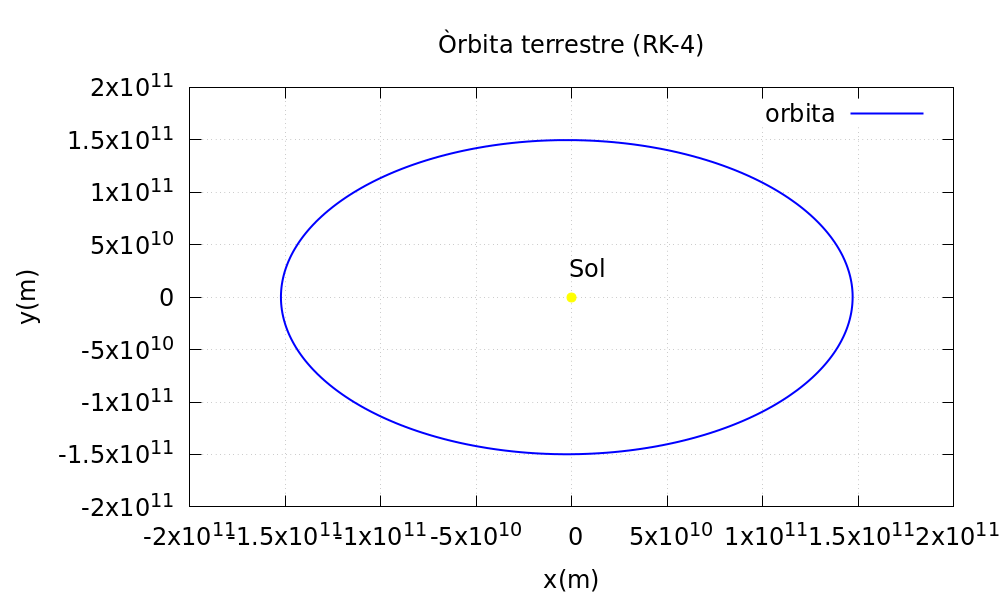
\includegraphics[width=\textwidth]{orbitaRK4.PNG}
        \caption{Òrbita terrestre per Runge-Kutta d'ordre 4}
        \label{fig: orbitaRK4}
    \end{subfigure}
    \caption{Càlcul òrbita terrestre per diferents mètodes numèrics}
    \label{fig: graficsRK}
\end{figure}

Calculem l'error acumulat en el radi orbital per poder veure millor les diferències entre resultats dels mètodes numèrics utilitzats.

\begin{equation}
    Error_{Eul} = \frac{\num{1.47098075136e11}-\num{1.47097294753e11}}{\num{1.47098075136e11}}100\approx0,00053052\%
\end{equation}

\begin{equation}
    Error_{RK2} = \frac{\num{1.47098075136e11}-\num{1.470972947846478e11}}{\num{1.47098075136e11}}100\approx0,00053049732\%
\end{equation}

\begin{equation}
    Error_{RK4} = \frac{\num{1.47098075136e11}-\num{1.470972947846474e11}}{\num{1.47098075136e11}}100\approx0,00053049732\%
\end{equation}

\section{Aproximació de la Terra a un esferoide}
\label{sec: terraesferoidedibuix}
En aquesta secció es mostren els passos per arribar a l'equació \eqref{rtel}.

Per una banda, el punt de la superfície de l'el·lipsoide es pot definir com:

\begin{equation}
    (x,y) = (acos(\xi),bsin(\xi))
\end{equation}

Partim de calcular el Radi de l'el·lipsoide amb el teorema de Pitàgores:

\begin{equation}
    R(t)^2 = a^2cos^2(\xi) + b^2sin^2(\xi)
    \label{eq: Pitagoreselipsoide}
\end{equation}

On $\xi$ és l'angle geocèntric. Però com les dades de posició de l'habitatge ens donen l'angle geodèsic $\epsilon$, ens interessarà relacionar-los per poder trobar la distància centre-superfície de la Terra per tenir en compte la nostra aproximació.

Obtenim l'equació que ens permet passar d'un angle a l'altre, \eqref{eq: alphatel}, a partir de trobar el pendent del vector normal $(x,y) = (bcos(t), asin(t))$ que a la vegada és la tangent de $\xi$.

\begin{equation}
    tan(\epsilon) = \frac{asin(\xi)}{bcos(\xi)} = \frac{a}{b}tan(\xi)
\end{equation}

El vector normal el podem obtenir girant 90º el vector tangent $(x,y) = (-asin(t),bcos(t))$ a la corba. Aquest últim l'hem calculat difernciant l'equació de la corba de l'el·lipsoide.

Això ho introduim a l'equació \eqref{eq: Pitagoreselipsoide} per obtenir l'expressió que utilitzarem per a recalcular el nostre radi, presentada en la secció \ref{sec: terranoesfera}.

\begin{figure}[H]
    \centering
    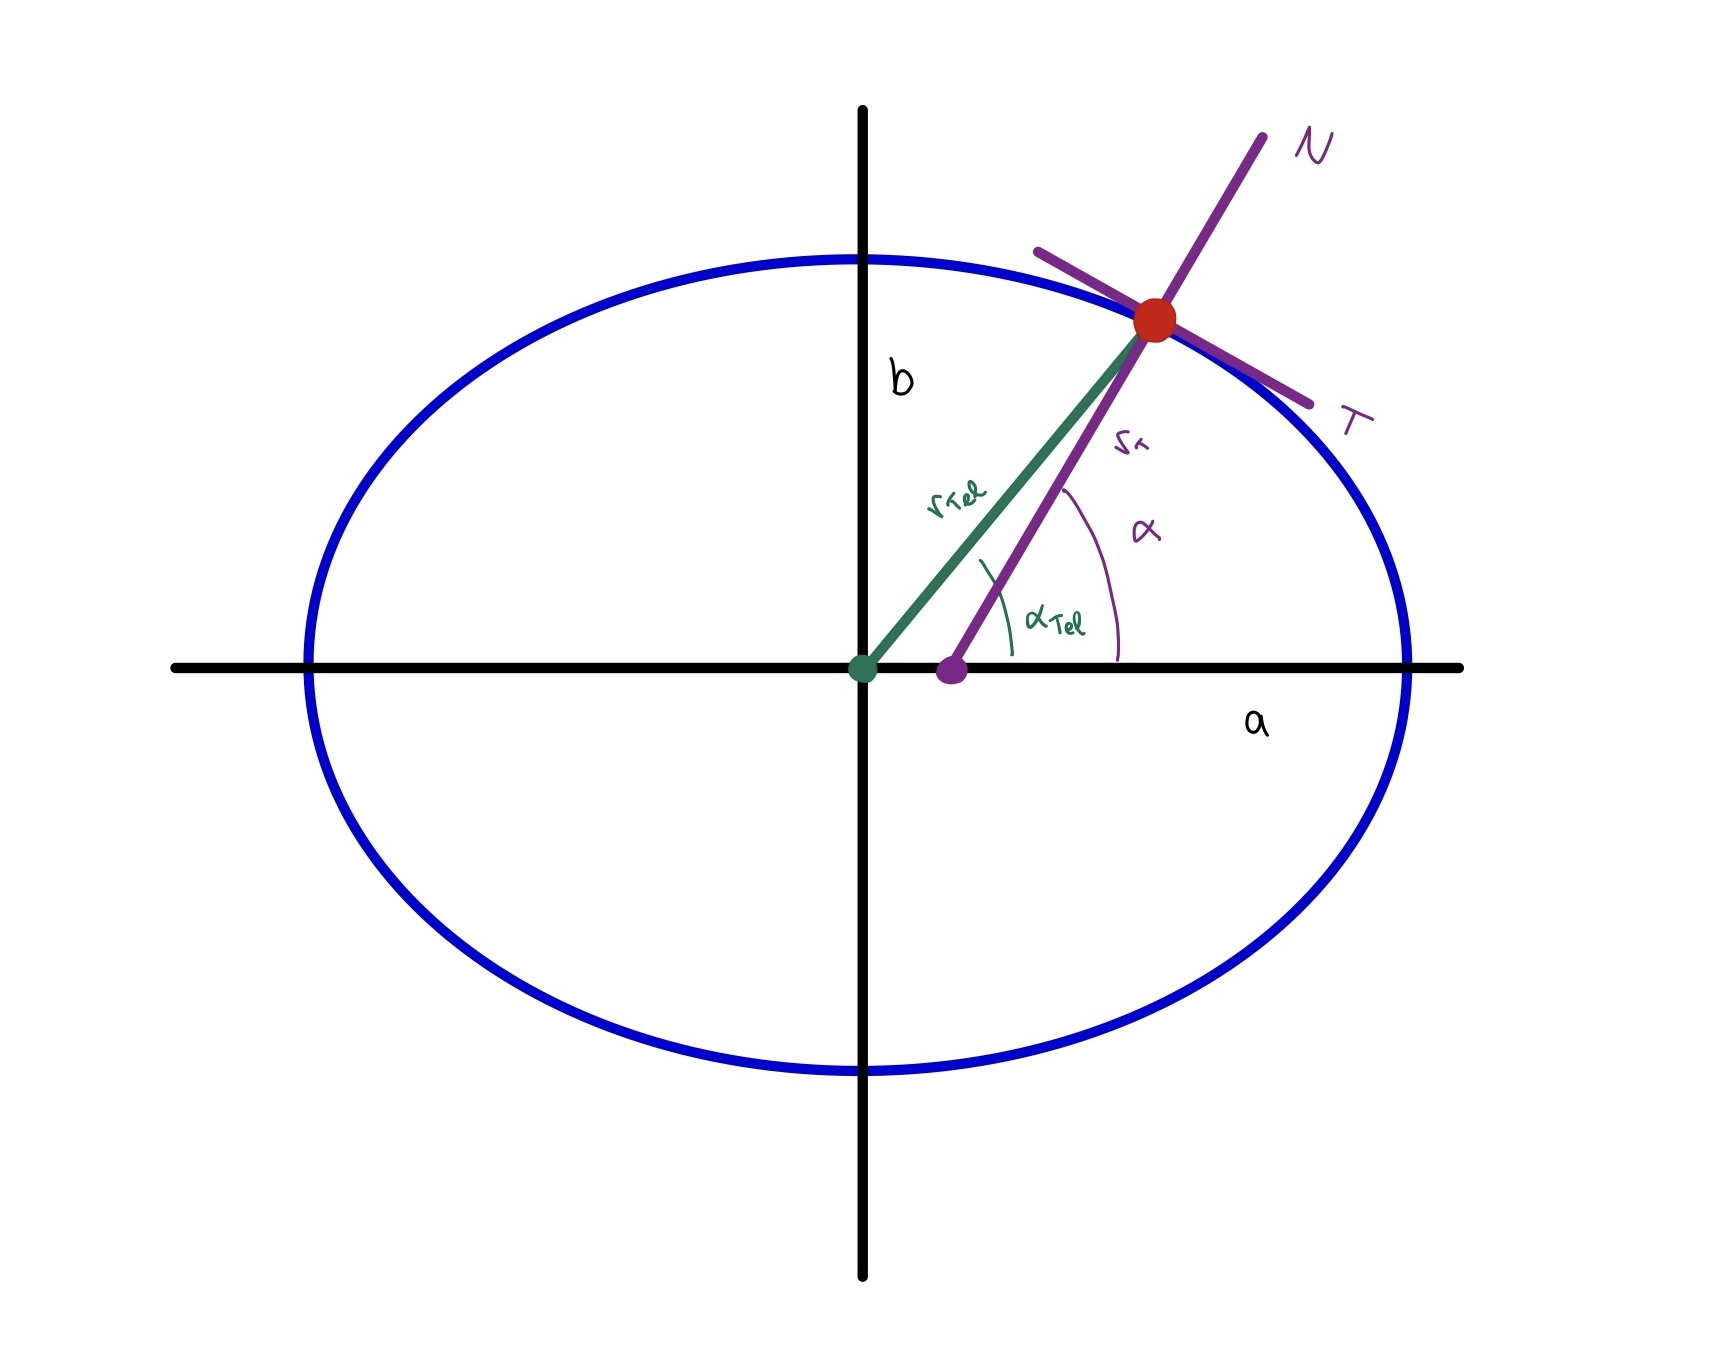
\includegraphics[width=0.5\textwidth]{Terraelipsoide.jpg}
    \caption{Aproximació de la Terra a un el·lipsoide de revolució, amb els angles i semieixos que hem d'utilitzat per recalcular el Radi Terrestre i l'angle de Latitud}
    \label{fig:terraelipsoide}
\end{figure}

En la figura \ref{fig:terraelipsoide}, l'angle $\xi$ correspon a $\alpha_{T_{el}}$ (l'angle geocèntric) i l'angle $\epsilon$ a $\alpha$ (l'angle geodèsic). Els semieixos que hem agafat per a calcular el radi de la terra com a una esferoide són a = 6378136.6 i b = 6356751.9, extrets de l'article de Viquikipèdia: El·lipsoide de referència.

\bibliographystyle{plain} % Estilo de bibliografía (puedes usar otros como unsrt, alpha, etc.)
\bibliography{bibliografia} % Nombre del archivo .bib sin extensión

\end{document}
